\section{High energy particles}

In this chapter, I will discuss the different types of high-energy particles that are of interest in this paper, i.e. neutrinos and ultra-high energy cosmic rays (UHECRs).
I will briefly discuss their generation and how they are detected. Then introduce how they lose energy in their journey to the Earth, and lastly calculate the emissivity of their hypothetical sources from the ground 
observations here on earth. 

\subsection{Acceleration of high energy particles}

To reach high energy, particles need to be accelerated. 
Knowing the exact source of acceleration can be difficult since we do not know the sources, but one can put constraints on any source given some simple arguments.
By arguing that the acceleration needs to be of a certain strength and that the particle being accelerated needs to stay confined within the accelerator for long enough one can put constraints on the source.
This is called the Hillas criterion  and is a way of estimating the maximum energy a particle can reach in a given source.% (ref hillas)

For relativistic particles with charge $Z$ and energy $\epsilon$ in a magnetic field of strength $B$ one can define the Larmor radius


\begin{equation}
    R_L = \frac{\epsilon}{ZB}
\end{equation}

By arguing that the definition of confinement of a particle to a source is by equating the Larmor radius to the size of the source one can 
easily derive the maximum achievable energy for a particle as follows.% (ref M. Bustamante. https://cds.cern.ch/record/1249755/files/p533.pdf)

\begin{equation}
    \epsilon_{max} = ZBR
\end{equation}

Via this method, one can illustrate the potential candidates needed to produce the required and importantly observed high-energy particles. 
This requirement is named the Hillas criterion after G. Hillas who first proposed this method\cite{Hillas_1984}.
The criterion works as an upper boundary of acceleration sources since it does not account for energy loss in the acceleration process or any type of interaction that one could expect to be in turbulent environments.
In figure \ref{fig:hillas_c} one can see the different candidates for the acceleration of two different ions, protons, and iron. One of the candidates is the AGN, which is the focus of this paper.

\begin{figure}
    \centering
    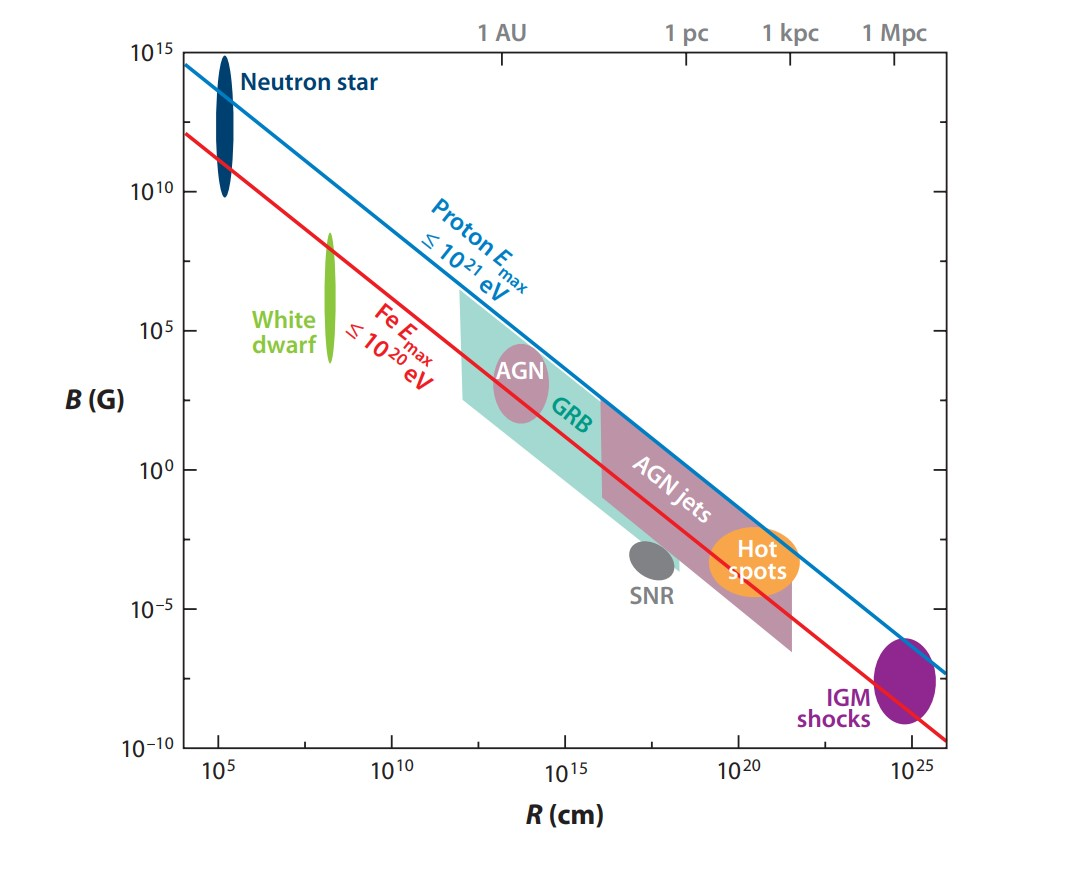
\includegraphics[width = 0.5\textwidth]{hillas_criterion.jpeg}
    \caption{Hillas criterion for proton (blue line) and iron (red line) accelerated up to $10^{20}eV$ and $10^{21}eV$ respectively. Image taken from \cite{doi:10.1146/annurev-astro-081710-102620}}
    \label{fig:hillas_c}
\end{figure}

The method of acceleration can be important for different sources. Here I will briefly go through some. 
\textbf{One-shot acceleration}:
In the presence of an ordered electric field, one can continuously accelerate charged particles. This could be the feature of some astrophysical objects such as neutron stars and black holes.% (ref cern paper)


\textbf{Diffusive acceleration/ Fermi acceleration}
In regions where one has high variability in the magnetic field strength, one can accelerate particles in steps. 
This is called diffusive acceleration and the most common way of this happening is through first and second-order Fermi acceleration.
The second-order Fermi acceleration is the simplest and is based on the fact that particles can gain energy by bouncing back and forth between magnetic clouds which act as mirrors. 
This is a stochastic process and the average energy gain can be shown to be proportional $(\frac{v}{c})^2$. Here $v$ is the speed of the cloud 
and $c$ is the speed of the particle. This is a slow process due to the scarcity of clouds, and therefore it is not a preferred method.
The first-order Fermi acceleration happens when particles collide with strong shock fronts. These shock fronts can be quite a bit faster than the interstellar clouds
and when a particle moves through the shock it gains energy proportional to $\frac{v}{c}$. In addition to this, there is a probability that the particle will stay in the accelerating region and 
experience several accelerations. 

By knowing how particles can be accelerated and their potential sources one can continue and look at the two particles in question in this paper. 
Neutrinos and UHECRs.
\subsection{UHECRs}

UHECRs are charged particles that are bombarding the Earth with energy exceeding 1 exaelectronvolt ($10^{18}$ eV) \cite{Alves_Batista_2019}. The origin of 
these particles is still a mystery but due to their high energies, they are thought to be extragalactic in origin and due to the Hillas criterion need to be sufficiently good accelerators.
The composition of UHECRs ranges from protons to heavier nuclei such as helium or iron, and when these particles interact with the atmosphere they produce a shower of secondary particles.
The air showers could also give extra information such as direction, but due to the nature of UHECRs, the location of their source is
difficult to pinpoint. This is because UHECRs are charged particles and therefore are deflected by the magnetic fields they encounter.

\subsubsection{Production and Energy loss}
The requirements to produce a UHECR are a charged particle and a powerful accelerator. But in order to
model them sufficiently one needs to take into account their journey to the Earth. Both during the acceleration and during the journey to Earth, the UHECRs will lose energy. 
The important parameters for this energy loss are its composition and its environment. In addition, as mentioned before, the interstellar magnetic field will also deflect the particles and therefore the direction of the particle will be changed. 
These effects are important parameters since they limit the 
distance a particle can travel before its initial energy becomes unreasonably large, and therefore limits the local volume in which it can be produced. 
Here I will briefly discuss the different energy loss mechanisms.

\textbf{Photo-pair production}

\begin{equation}
    p + \gamma \rightarrow p + e^- + e^+
\end{equation}

For UHECRs, the most dominant sink of energy for when at relatively low energy is the Bethe-Heitler process. In this process, a proton of sufficient energy interacts with the 
photon field in its vicinity and produces a pair of electrons and positrons. The photon field can vary from the cosmic microwave background to the generated field from different sources. 
The energy loss of this process is quite small $\sim \frac{2m_e}{m_p}= 10^{-3}$ of the original energy of the proton, but the process is very common, and therefore it is a significant energy loss over time.


\textbf{Photo-Pion production }
\begin{equation}
    p + \gamma \rightarrow \Delta^+ \rightarrow (p + \pi^0)\quad \text{or} \quad (\pi^+ + n)
    \label{eq:delta_resonance}
\end{equation}

Given enough energy the proton can interact with the photon field and produce a delta resonance. This resonance can then decay into a pion and a proton or a neutron and a pion. 
It is important since it also puts an upper limit on the UHECR energy for intergalactic particles. 
This limit, called the Greisen-Zatsepin-Kuzmin (GZK) limit comes from the UHECRs interacting with the cosmic microwave background in this delta resonance process. The limit caps proton energy at $5\times 10^{19}$ eV.
In this mechanism the original proton loses $m_p/m_\pi \approx 20\% $ of its energy resulting in a quite rapid loss of energy.

%\textbf{photodisintegration}
%mabye include this. 



%https://inspirehep.net/literature/1611251
% https://journals.aps.org/prl/abstract/10.1103/PhysRevLett.125.121106


\subsubsection{Detection}
When a cosmic ray hits the atmosphere it will interact with the air molecules and produce a cascade of particles and light that can more easily be detected than 
the original cosmic ray. In addition, since the UHECR flux at high energy is extremely low ($<$1 particle per $\rm km^2$ per year for $E > 10^{19}$) one needs a large area to collect enough data. 
The largest UHECRs detectors of present are the Pierre Auger Observatory and the Telescope Array. 

The Pierre Auger Observatory is located in Argentina and is the largest detector of its kind. It consists of 1660  Cherenkov detectors spread over 3000 km$^2$ and 27 fluorescence telescopes in four locations. With 
these instruments, the observatory is very capable of reconstructing the air showers and therefore the energy and direction of the cosmic ray. The observatory has a blind spot in the night sky 
and therefore the observatory is complemented by the Telescope Array located in Utah. The Telescope Array is a smaller observatory with 507 scintillator detectors and 3 fluorescence telescopes. Combined they have been able to map the full sky of UHECRs.  

\subsubsection{Emissivity estimates}
\label{sec:emmisivity}

Now that one reasonably understands the nature of UHECRs one can try to make tangible estimates of the UHECR sources. One such
estimate is the emissivity of UHECR sources. The emissivity is a measure of the energy released per unit time per unit volume. The question 
one can ask is what is the necessary emissivity of UHECRs to explain the observed flux here on Earth? In other words, what is the required energy injection rate of UHECRs?


\begin{figure}
    \centering
    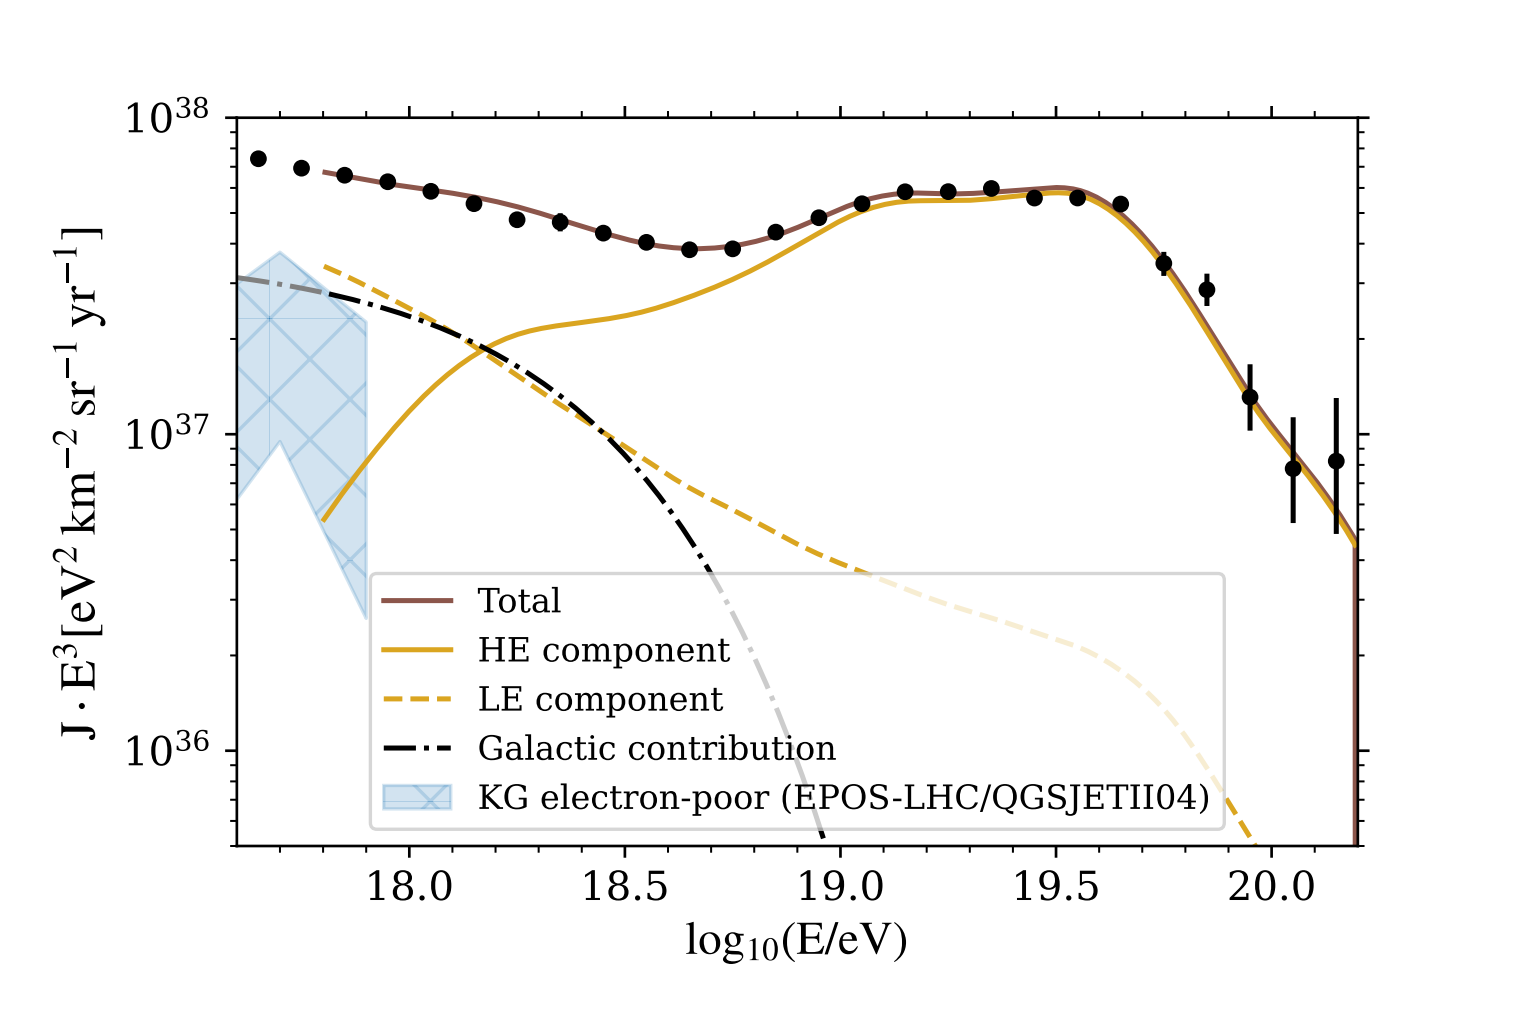
\includegraphics[width = 0.7\textwidth]{UHECRs.png}
    \caption{The diffuse flux of UHECRs as measured by the Pierre Auger Observatory and the Telescope Array. The flux is separated into galactic and extra galactic sources where the total spectrum follows the black dots. Image taken from \cite{Abdul_Halim_2023}}
    \label{fig:flux_UHECRs}
\end{figure}

Via observations from the Pierre Auger Observatory and the Telescope Array, one can observe and model the diffuse flux of UHECRs. The result is an isotropic flux and is represented in Figure \ref{fig:flux_UHECRs}.  By separating the 
flux into contributions from extragalactic sources and galactic sources one can estimate the required energy density in the Universe of extragalactic UHECRs. From here can define an energy loss time for a UHECR as the loss length divided by the speed of light $c$.
 The loss length is a measure of the distance a UHECR can travel before its energy drops below a certain threshold, and for our simple analysis, we will use the length of $1 Gpc$. This number is comparable in magnitude
as found by \cite{Stanev_2009} but as the loss length is dependent on initial energy and composition our number will be an approximation. 
Then the emissivity of UHECRs produced by the sources as the energy density divided by the loss time.

The previous discussion is summarized in the following equation 

\begin{equation}
    \epsilon_{\rm UHECR} = \frac{u_{\rm UHECR}}{t_{\rm loss}} = \frac{u_{\rm UHECR}}{D_{\rm loss}/c} = \frac{4\pi c \int_{E_0}^{E_{\rm max}}J_{\rm extragalactic}(E)E dE}{c D_{\rm loss}} \approx 9\times 10^{44} \frac{\rm erg}{\rm Mpc^3 \rm yr}.
\end{equation}

Here $u_{UHECR}$ is the energy density of UHECRs, $t_{loss}$ is the energy loss time, $D_{loss}$ is the loss distance, $J(E)$ is the flux of UHECRs, $E_0$ is the minimum energy of the flux where it is dominated by extragalactic UHECRs, and $E_{max}$ is the maximum energy of extragalactic UHECRs.
The value of $\epsilon_{UHECR}$ is calculated in the script available on GitHub \cite{Andrews_2023_github} by using data from  Auger \cite{thepierreaugercollaboration2017pierre}. This emissivity is a crude estimation of the required energy injection rate of UHECRs and is meant to give a rough estimate. 
The main points of criticism are the estimate of our loss distance which does not include the composition of the UHECRs or its initial energy. Nevertheless, one receives an emissivity comparable to a more thorough analysis from \cite{PhysRevLett.125.121106} which received a value of $6*10^{44} \frac{\rm erg}{\rm Mpc^3 \rm yr}$.




\subsection{Neutrinos}

The second particle of interest is the neutrino. Neutrinos compared to UHECRs are neutral particles that are produced in various processes in the Universe.
The most common and well-known is the fusion reaction in the sun where neutrinos are produced in the pp chain. On the other hand the neutrinos of focus in this paper 
are high-energy neutrinos that are likely produced in the same sources as the UHECRs.



\subsubsection{Production and Energy loss}
The production sites of high-energy neutrinos is not clear, but they are thought to be produced in the same sources as UHECRs 
and in this section, I will go through the most probable way of producing high-energy neutrinos in sources such as AGNs.

\textbf{Hadronic processes}:

Hadronic processes can release neutrinos with sufficiently high energy to explain the observations here on Earth. 
Processes such as nuclear interactions are limited by the binding energy of the nucleus and accelerating a neutrino after its production is difficult.
Therefore, a common way of producing the observed neutrinos is through the decay of pions. The most important decay is the decay of charged pions into muons and muon neutrinos as seen in \ref{eq:pion_decay}


\begin{equation}
    \pi^+ \rightarrow \mu^+ + \nu_\mu \rightarrow e^+ + \nu_e + \nu_\mu + \bar{\nu_\mu}
    \label{eq:pion_decay}
\end{equation}

I will discuss two possible ways of producing these pions in two different environments. 


In a proton-rich environment where the protons can accelerate up to high energies, one can produce pions through the following process
\begin{equation}
    p + p \rightarrow \begin{cases}
        \pi^+ + n+ p \\
        \pi^- + \pi^+ +p + p  \\
        \pi^0 + p+p
    \end{cases}
\end{equation}

The energy of these protons at a few GeV is enough to introduce the delta-baryon resonance, and therefore it becomes more complicated.
The most efficient way of producing pions is through the already seen delta resonance when a proton interacts with a photon \ref{eq:delta_resonance}.
This process being the cooling process of UHECRs above the GZK limit is interesting and indicates that a source that produces high energy neutrinos likely is inhabited by very energetic charged particles. 
After having produced the neutrinos it also becomes important to understand their behavior during their travel to Earth. Here I will highlight two points


\textbf{Neutrino oscillations}
In the previous paragraph, I discussed the production of these neutrinos, but not their initial flavor.
The pion decay model is known to produce a flavor composition of $\nu_e : \nu_\mu : \nu_\tau = 1:2:0$. 
A naive thought would be an identical composition observed on Earth, but sadly this is not the case. 
The reason for this is that the neutrinos' mass state can oscillate between the different flavors. Therefore, the neutrinos produced in the source will oscillate during their travel to Earth and when they reach us one would expect a 
uniform mix of the three flavors, $\ nu_e: \nu_\mu: \nu_\tau = 1:1:1$.

\textbf{Energy loss}
To model the travel of a neutrino of any flavor one only needs to take into account the interaction of the neutrino with the expanding universe. Since it is so weakly interacting the only 
source of energy loss the flux of neutrinos will experience is the redshift created by the expansion of the Universe. This redshift is the same as the one discussed in the previous section and the neutrinos 
behave the same way light does in this manner with a drop in energy proportional to $(1+z)$.



 

\subsubsection{Detection}
\begin{figure}
    \centering
    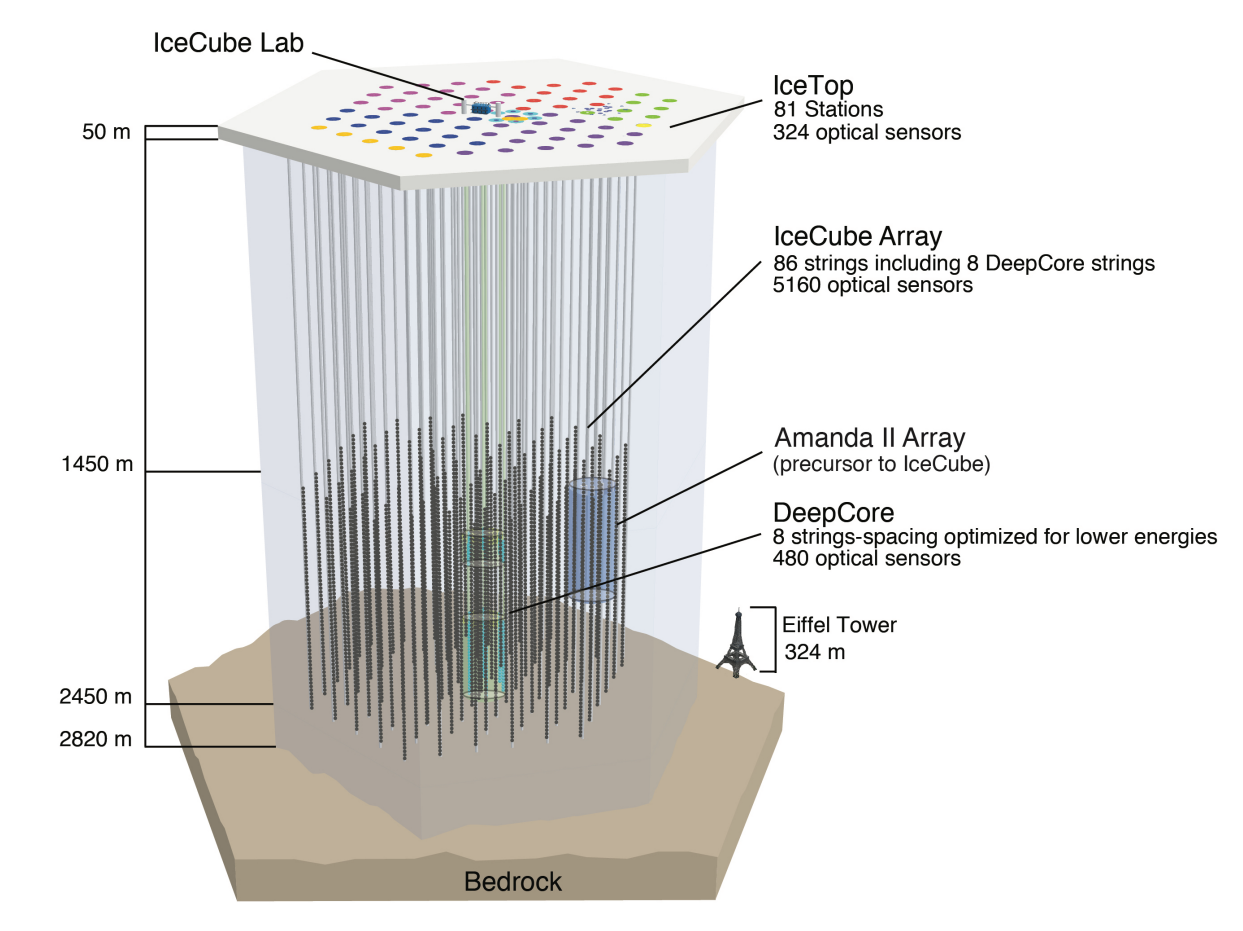
\includegraphics[width = 0.5\textwidth]{Ice_cube_layot.png}
    \caption{The IceCube neutrino observatory. The detector is located at the South Pole and is a large block of ice instrumented with photomultiplier tubes. Image taken from \cite{Andeen_2019}}
    \label{fig:Ice_cube}
\end{figure}

Neutrinos are weakly interacting matter particles and therefore are very difficult to detect. This makes them excellent candidates for the study of the Universe since they can travel large distances without interacting, but make them 
quite difficult to detect with high accuracy. The most famous detector and the one used in this paper is the IceCube neutrino observatory. This detector is precisely what it sounds. It is a large block of ice with a size equal to a square kilometer located at the South Pole.
The observatory uses the ice located deep in the South Pole as a giant Cherenkov detector. The ice is instrumented with photomultiplier tubes that can detect the Cherenkov radiation produced by neutrinos interacting with the ice. 
More precisely the observatory is fitted with 5160 photomultiplier tubes located at a depth of 1450-2450 m. The photomultipliers are divided into 86 strings of 60 modules each. The detector is also complemented by the DeepCore detector which is a denser array of photomultiplier tubes located in the center of the detector. See Figure \ref{fig:Ice_cube} for a visual representation of the detector.
The energy range for this detector is from 10 GeV to 10 EeV. The interaction of neutrinos with the water molecules in the ice can produce charged leptons (muons, electrons or taus). These charged particles if energetic enough will then produce Cherenkov radiation which can be detected by the photomultiplier tubes.


\subsubsection{Emissivity estimates}
\label{sec:emmisivity_neutrinos}

Armed with the required knowledge above one can also make simple arguments for the sources of these neutrinos based on the observed 
flux here on Earth. The flux used in this paper is the diffuse flux of neutrinos as measured by the Ice Cube observatory. The flux is shown in figure \ref{fig:flux_neutrinos}. 
For any calculations, we use the astrophysical flux as modeled as a power law. The power law is of the form 

\begin{equation}
    \Phi(E) = \Phi_0 \left(\frac{E}{E_0}\right)^{-\gamma}
\end{equation}

with $\Phi_0$ being the normalization constant, $E_0$ being the reference energy and $\gamma$ being the spectral index. The model parameters are seen in table \ref{tab:neutrino_flux} and taken from \cite{Abbasi_2022}.

\begin{table}
    \centering
    \begin{tabular}{|c|c|c|}
        \hline
        $\Phi_0$ & $E_0$ & $\gamma$ \\
        \hline
        $6.7\times 10^{-18} GeV^{-1} cm^{-2} s^{-1} sr^{-1}$ & $100 TeV$ & 2.37 \\
        \hline
    \end{tabular}
    \caption{The model parameters for the astrophysical flux of neutrinos as measured by the Ice Cube observatory.}
    \label{tab:neutrino_flux}
\end{table}

The emissivity of neutrinos is calculated in the same way as for UHECRs. The only difference is the loss time. Neutrinos do not lose energy in the same way as UHECRs and therefore the loss distance will be the size of the Universe. 
The modeled emissivity is then approximately $1.54 10^{44} \quad erg/Mpc^3/yr$. 

\begin{figure}
    \centering
    \begin{subfigure}[b]{0.35\textwidth}
        \centering
        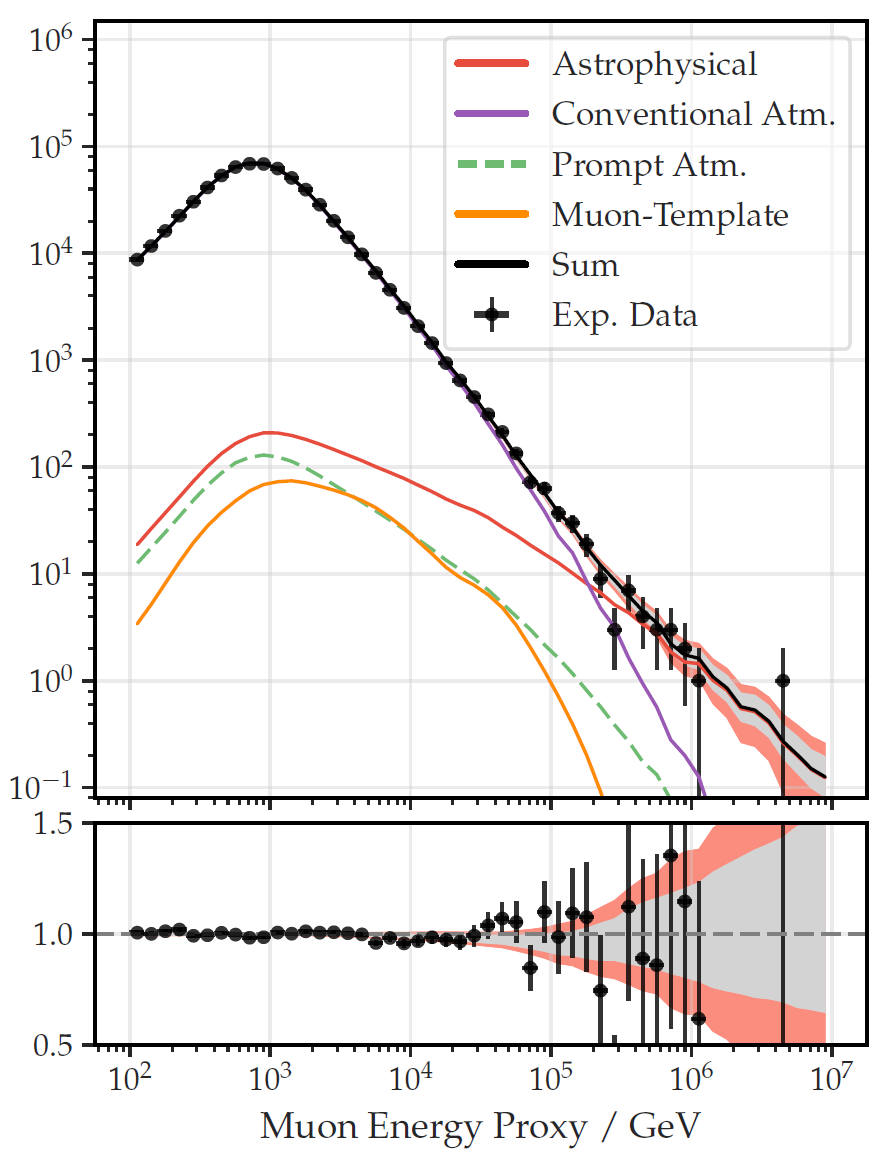
\includegraphics[width=\textwidth]{Ice_cube_flux_tot.png}
        \caption{Number of events per bin}
    \end{subfigure}%
    \begin{subfigure}[b]{0.5\textwidth}
        \centering
        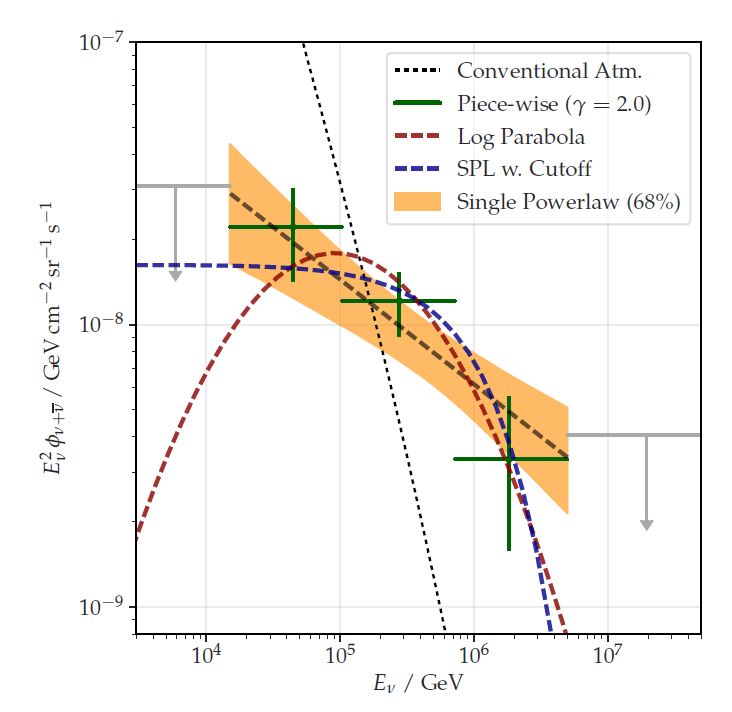
\includegraphics[width=\textwidth]{Ice_cube_flux_astro.png}
        \caption{Modeled Astrophysical flux}
    \end{subfigure}
    \caption{The diffuse flux of neutrinos as measured by the Ice Cube observatory. The y-axis on the left image is the number of events per bin.  The flux is separated into contributions from atmospheric neutrinos and astrophysical neutrinos. The right image is the model astrophysical flux as measured by ICE CUBE. Images taken from \cite{Abbasi_2022} }
    \label{fig:flux_neutrinos}
\end{figure}


